\documentclass{ctexart}
\textheight 23.5cm \textwidth 15.8cm
\topmargin -1.5cm \oddsidemargin 0.3cm \evensidemargin -0.3cm

\usepackage{verbatim}
\usepackage{fancyhdr}
\usepackage{float}
\usepackage{graphicx}
\usepackage{amssymb}
\usepackage{amsmath}


\pagestyle{fancy}
\CTEXsetup[format = {\Large\bfseries\it}]{section}


\begin{document}

\section*{内容简介}
	\noindent 在计算机中心程序苦衷寻找一个适合求解一阶常微分方程系统初值问题的程序,利用此程序求解下列问题:
	\begin{equation}
	\begin{cases}
		\dfrac{dx}{dt} = \sin x + \cos yt \qquad x(-1) = 2.37 \\[5mm]
		\dfrac{dy}{dt} = e^{-xt} + \dfrac{\sin yt}{t} \qquad y(-1) = -3.48
	\end{cases} 
	\end{equation}
	在区间 $[-1,\,4]$ 上的阶要求具有 8 个小数位的精度。在 $t$ 轴上以 0.1 的间隔打印解。
	\begin{itemize}
		\item 对 $-1 \leqslant t \leqslant 4$,得到函数 $x(t)$ 和 $y(t)$ 的图表。两条曲线应该出现在同一个图表上。
		\item 得到下列参数定义的曲线图
		\begin{gather*}
			\{ (x(t),\,y(t)) : -1 \leqslant t \leqslant 4 \}
		\end{gather*}
		($t$ 的值不出现在图中。)这里得到的曲线称为原微分方程的轨道。
	\end{itemize}
	
	
\section*{工作环境}

	程序所用语言: {\bf python}
	
	软件: {\bf JupyterLab}
	
	使用的包: {\bf numpy, matplotlib, bisect }

\section*{输出结果}

\begin{figure}[H]
	\centering
	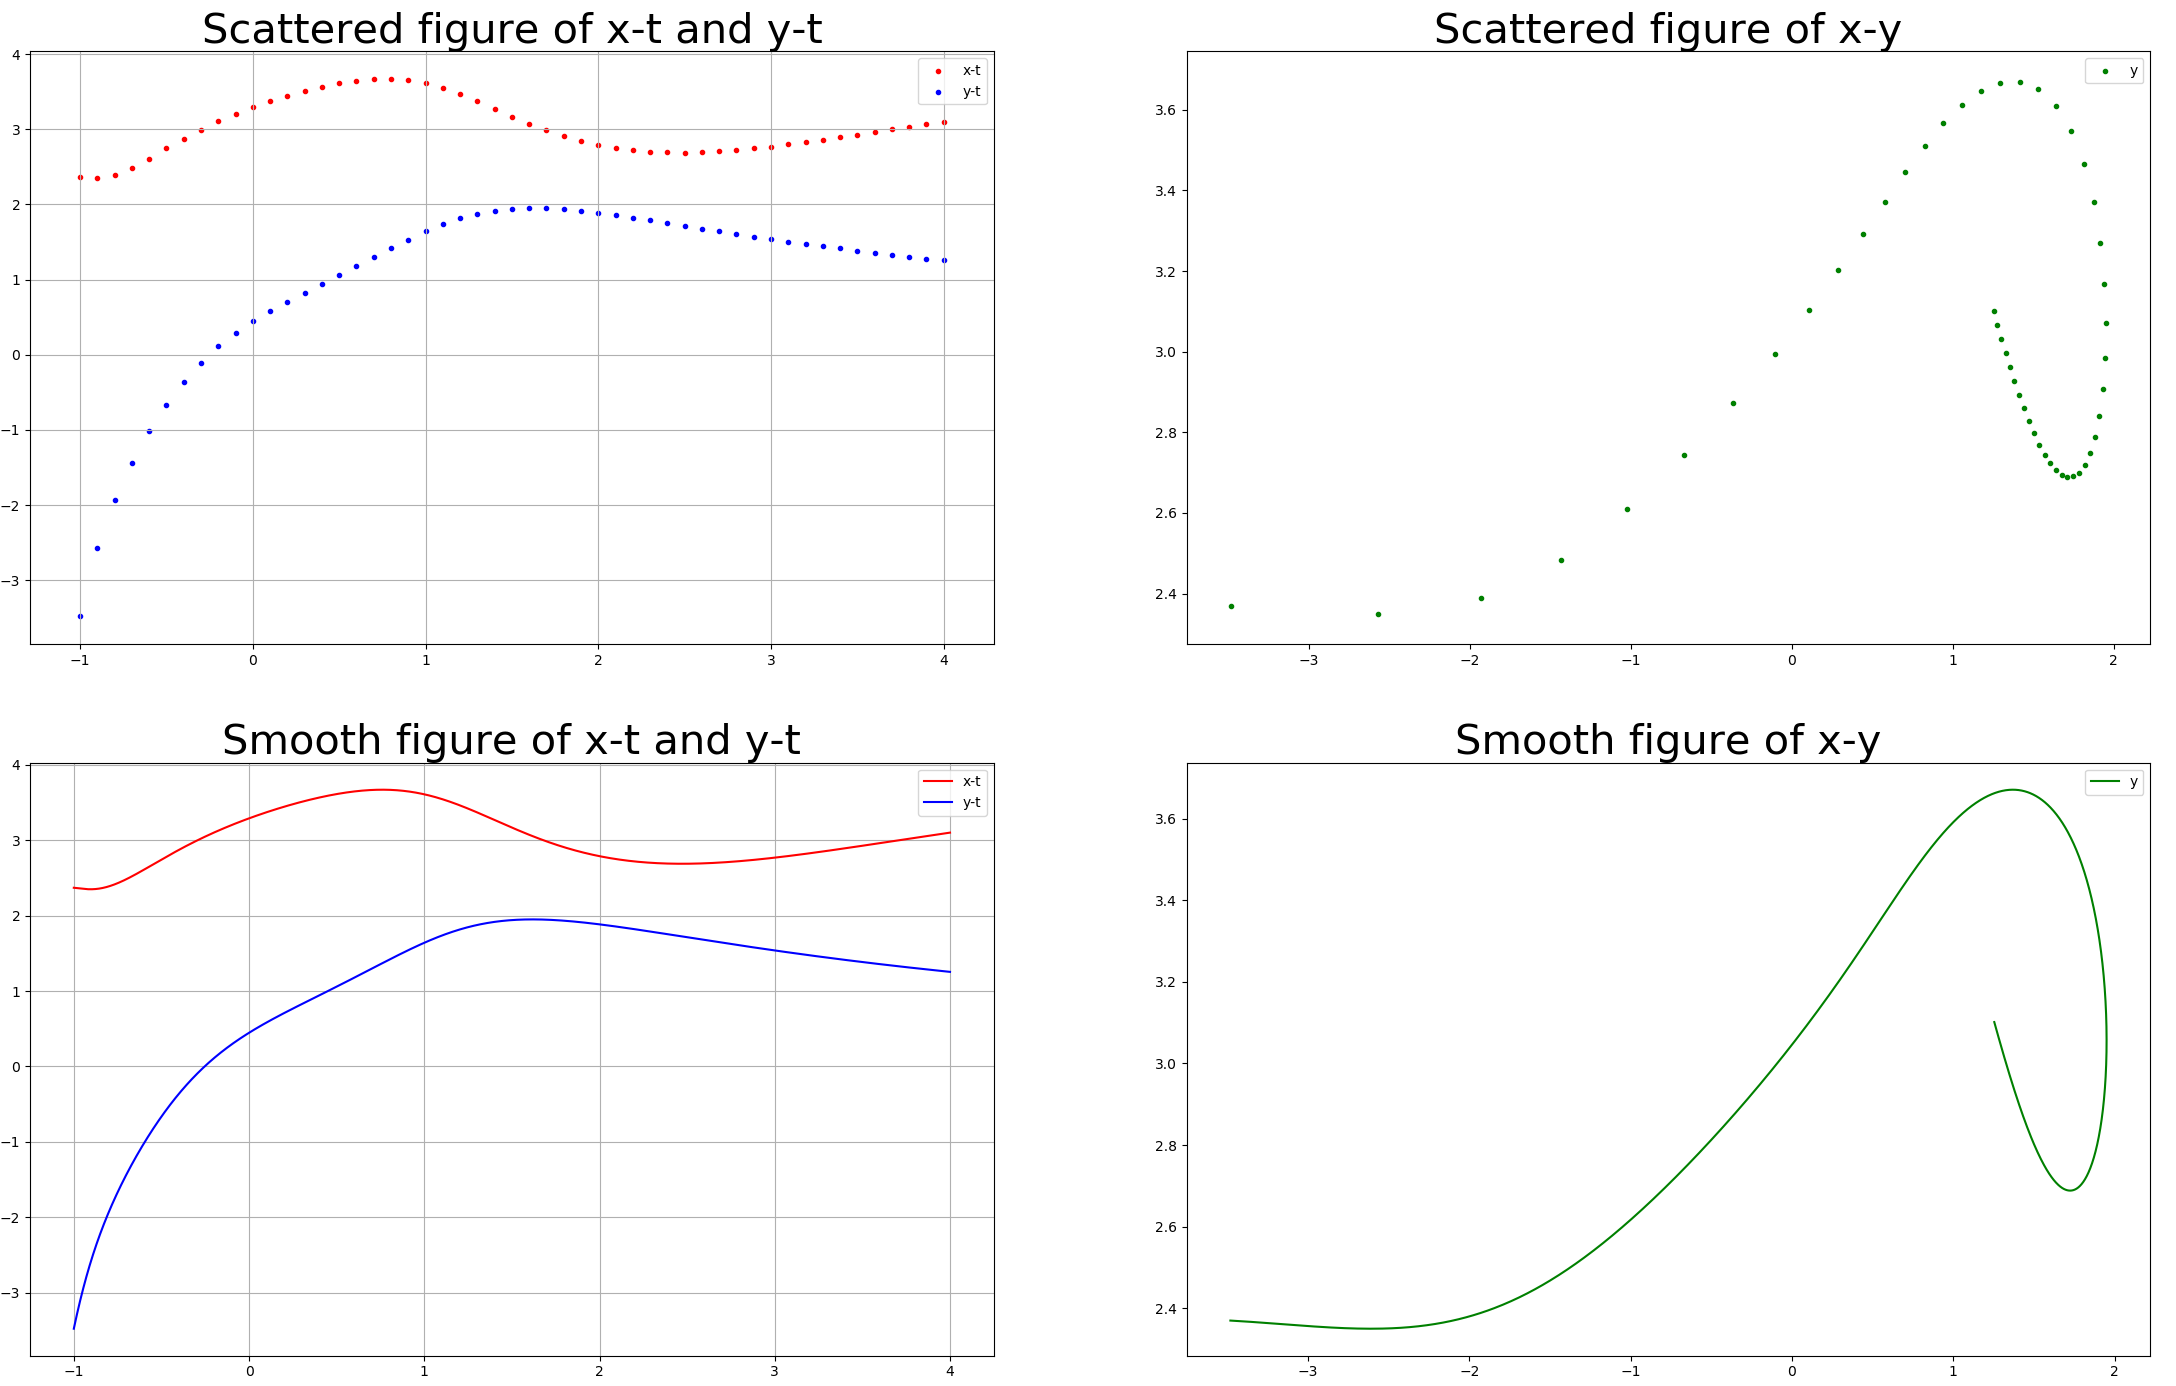
\includegraphics[width = 15cm, height = 8cm]{figure.png}
\end{figure}
	左侧图表横轴为 t,纵轴为 x 及 y。 右侧图表横轴为 x,纵轴为 y。

\section*{分析}
	\noindent 一、使用的方法及其精度控制
	
	本报告中显示的输出是来自自适应 RKF54 方法、初始步长为 $0.001$ 的结果。 自适应 RKF54 方法的是收敛的,并具有步进误差可控,自动调整步长的优点。这里设误差阈值为 $10^{-16}$,使得单步误差远低于题中要求的 8 个小数位。这里结合了课程中提到的两种控制误差的方式,并且将重新计算不合适的步长(此处“不合适”被理解为超过给定阈值两倍)。步长调整部分的代码如下:
	\begin{figure}[H]
		\centering
		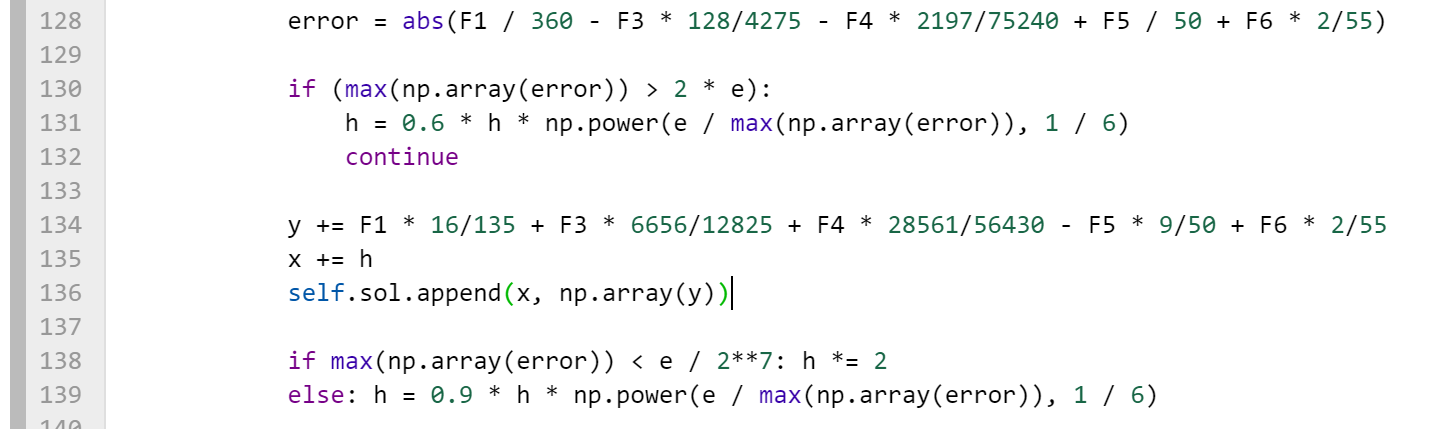
\includegraphics[width = 14cm, height = 4cm]{handle-error.png}
	\end{figure}

	这里重新计算步长虽可能导致程序死循环,但因容易处理,并且本例中未发生该情况,同时为了提高一些效率,便不加入处理该情形的相关代码。
	
	因 python 面向对象的特性,利用前几次程序作业的代码,本次提交的程序中方便的实现了能够求解该方程的其他几个方法(五阶 Runge-Kutta 方法、五阶 Adams-Bashforth 方法、五阶 Adams-Bashforth-Moulton 预估校正方法)。并且它们都可用于其它任意阶微分方程组的数值求解。只需修改代码第 26 行所调用的函数即可。注意其他非自适应方法不需要提供误差阈值。
	\begin{figure}[H]
		\centering
		\includegraphics[width = 10cm, height = 2cm]{capture.png}
	\end{figure}
	
	\noindent 二、所求解方程的性质
	
	原方程组为:
	\begin{equation}
		\dfrac{d}{dt} X = \dfrac{d}{dt}\begin{pmatrix}
			x\\y
		\end{pmatrix} = \begin{pmatrix}
			\sin x + \cos yt \\
			e^{-xt} + \dfrac{\sin yt}{t}
		\end{pmatrix} = F(t,\,X)
	\end{equation}
	
	因 $\displaystyle\dfrac{\partial}{\partial y}\dfrac{\sin yt}{t} = \cos yt$,故对于 $t \in (-1,\,4)$,$X \in (0,\,+\infty) \times (-\infty,\,+\infty)$,易知有
	\begin{equation}
		\Big\Vert F(t,\,X_1) - F(t,\,X_1)\Big\Vert_2 \leqslant 2(e+1)\Big\Vert X_1 - X_2\Big\Vert_2
	\end{equation}
	
	进而由初值问题解的存在唯一性定理知原常微分方程在 $(t,\,X) \in (-1,\,4) \times (0,\,+\infty) \times (-\infty,\,+\infty)$ 上的解存在唯一。
	

\section*{参考资料}
	\noindent [1] David R. Kincaid \& E. Ward Cheney. {\it Numerical Analysis: Mathematics of Scientific of Computing Third Edition}, Brooks/Cole, 2002.

\end{document}